\documentclass{article}
\usepackage[utf8]{inputenc}
\usepackage{microtype}
\usepackage{graphicx}
\usepackage{wrapfig}
\usepackage{lscape}
\usepackage{rotating}
\usepackage{epstopdf}

\title{Making a Pong game based on an MSP430}
\author{Sergio Mauricio Guerrero Gaona (smg10) \\ Ben Gruber (bpg1)}
\date{April 2019}

\begin{document}

\maketitle

\section{Motivation}
Throughout the semester we've been exploring the ins and outs of designing and implementing embedded systems. We've written
several drivers for the MSP430's modules and integrated them with software logic to make interesting devices that that interact with the real world while meeting tight timing considerations. This semester, the culmination of all of our labs was the
Simon project. We put together all of our code from the semester and wrote complicated logic to implement a fun game! This was
the source of our motivation to build another game. We enjoyed writing the Simon software and wanted to dive deeper into games
running on embedded systems. Another driving force was the goal of integrating a graphic display panel into our design. We
explored several ideas and finally decided on making a Pong replica!

\section{System Specification}
The Pong game is the arcade classic with two paddles on either end of the screen controlled by users and a ball that is bounced between the paddles and the top and bottom of the screen. If the ball makes it to either end of the screen, a point is scored. The paddles were originally controlled with knobs. 

Since we wanted to make a close replica of the game we ended up choosing potentiometers for paddle control, a black and white OLED panel (to get a CRT-esque feeling), and a couple of buttons for basic interaction.

For software this meant that we needed to implement drivers for GPIO, ADC, and the screen. The game logic required that we implement (but not limit ourselves to) collision checking, bouncing, scoring, ball movement, and detecting winners.
\pagebreak

\section{Parts Selection}
The main parts of our system are the potentiometers, the OLED display panel, and the pushbuttons.

Potentiometers can be used to generate an analog signal dependent on a physical position of the device. This analog signal controls the position of the paddles on the screen.

In choosing the resistance for our potentiometers, we needed to find a middle ground between power consumption and the allowed sampling time
on our ADC. A higher potentiometer resistance decreases the resistive current draw from $V_{dd}$ to ground, but increases the time constant on the ADC pin, which decreases the maximum allowed sampling rate. This corresponds to a trade-off between battery life and potential control lag.
Factoring in both performance and availability, we settled on a resistance of 22 k$\Omega$ for each of our potentiometers. At 22 k$\Omega$ the current flowing across the of the potentiometers is 0.15 mA. This is quite small compared to the estimated 10-20 mA consumption of the display, and thus has unnoticeable effects on power consumption. The ADC10 on the MSP430 requires at least 5 $\mu$s to sample the voltage of a source with 22 k$\Omega$ of impedance.
Thus, power consumption is minute and sampling times do not introduce any noticeable lag.

Our system has a total of 3 pushbuttons. One is used as a hardware reset and the others are used as GPIO inputs. The GPIO buttons are used as user input for advancing the game's sate. We opted for an active low configuration with no hardware debouncing.


Over the semester we implemented a driver for the MSP430 to operate as an SPI master. Because of this, and the high speed nature of SPI, we decided to search for an SPI controlled screen. We gravitated towards a monochrome OLED panel because of how crisp and bright they look, opting for black and white to mimick pong as much as possible. The screen we ended up selecting is a 128x64 OLED panel that communicates over 3-wire SPI. The controller also has a Data/Command line that determines what is being sent over the bus. Commands are used for initialization, inverting the display, moving the cursor, etc. Data corresponds to the bytes that are written to the location in the controller's memory that is pointed to by the cursor. This memory on the driver corresponds to the data that is seen on the screen.

The basic operation of the screen involves writing to pages of the memory buffer on the OLED driver. The organization of the buffer in the driver is shown in figure 1 below. Consider Page 0 and SEG0. This memory location corresponds to the 8 pixels located at $x=0$ and $0<y<7$. Similarly, Page 7 SEG127 corresponds to the 8 pixels located at $x=127$ and $56<y<63$. Now, say you want to turn on the pixel at position $(x,y)$. You need to determine three things: SEG number, Page number, and location of the pixel within Page number.
SEG simply corresponds to the $x$ position you want to write. You can then determine Page number by $page_{no} = y/8$ (using integer division). Then, the position of $y$ within the page is determined by $offset = y-8*page_{no}$. With this information, you move the controller's data pointer (cursor) to the location $(x, page_no)$ and write the byte with bit $offset$ set to that location.

Using the above routine to turn on single pixels, we wrote more advanced routines to draw rectangles of arbitrary size on the screen. The rest of the OLED software is discussed in the Software section.

\begin{figure}[h!]
    \centering
    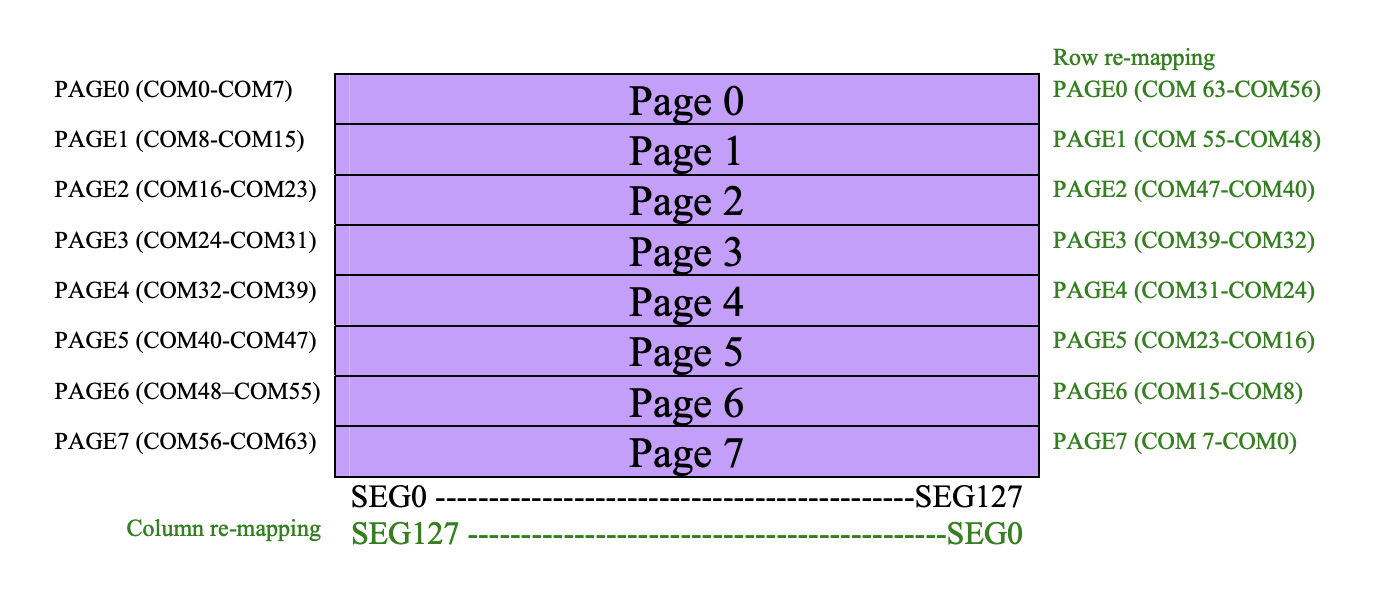
\includegraphics[width=\textwidth]{buffre.png}
    \caption{SSD1306 Controller Memory Organization}
    \label{fig:my_label}
\end{figure}

 In the design of our system we chose to use 4 AA batteries in series for a total supply voltage of 6 V. We chose this in order to give our screen plenty of voltage to achieve good brightness for our game. This meant that we needed to step down those 6 V to 3.3 V. For that we chose the Traco TSR 1-2433 switching power regulator. This part acts as the power supply to our MSP430 when the system runs off of battery power. Through performing theoretical analysis based on our finished product's measured power consumption, we determined that our system can run continuously for 11 days on a single set of 4 AA batteries. Since a game of pong takes only a few minutes, we expected battery longevity not to be an issue.


\section{System Architecture}
\subsection{Hardware}

Figure 2 below shows the block diagram for our system. This high level diagram allowed us to brainstorm ideas and have a very clear road map when going into the schematic design. It was also useful for writing software since it pinpoints the hardware dependencies of each of our components.

\begin{figure}[h!]
    \centering
    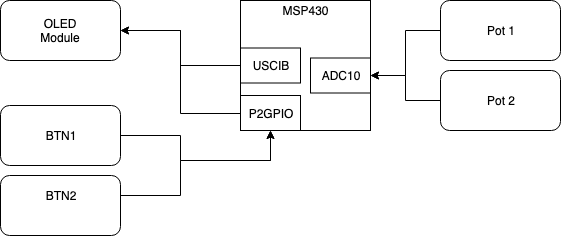
\includegraphics[width=\textwidth]{diag.png}
    \caption{HW block diagram of Pong}
    \label{fig:my_label}
\end{figure}

The schematic is in 7 after the end of the document. We followed the standard design patters we learned throughout the semester. One thing to note is the power selection jumpers. These jumpers allow us to change the power supplies for the MSP430 and the OLED module independently. The MSP430 can be powered from the launchpad, from the discrete regulator, or from the onboard regulator on the OLED module. The OLED can be powered from the launchpad, from the 6 V battery pack, or from the discrete regulator. We chose to add these jumpers for two reasons. We wanted the ability to isolate power supplies that were not in use, and we wanted to test the system under different configurations using the available supplies.
These jumpers proved to be useful during software development because the device could be running off of battery power while getting plugged in to our computers back and forth. 

Lastly our layout is in figure 8. We chose to spread out the potentiometers and buttons to give the players ample space to interact with the game simultaneously while focusing on the screen in the center. This also allows the game to be played with the players facing each other!

\subsection{Software}
We maintain our game state by tracking the position and velocity of the ball in the x and y directions, as well as the vertical position
of each paddle. In addition, we keep track of each player's score. On each iteration of the game loop, we update the vertical
height of each paddle by mapping the corresponding potentiometer position to a display position. We then update the position of
the ball by adding the velocities
to their corresponding positions, constraining the position of the ball so it remains on the screen at all times. In the
event that the ball is at the top of the screen, we negate its y velocity, and in the event that the ball is on one of the paddles, we negate
its x velocity, adding a random component to the y velocity to liven things up. If the ball goes past a paddle,
the round of the game is terminated and the opposite player is awarded a point. When a player reaches 9 points they are declared the winner.

In order to make drawing to the display as fast as possible, we separate the code that calculates the positions of the ball
and paddles from the code that draws them, placing the calculations before the drawing.

In the spirit of good software design, we sought to make our code modular. We thus have different modules for controlling the potentiometers, the buttons, the game logic, and the display. This design allowed us to expose a minimal amount of global variables and functions between modules to minimize the propensity of deeply hidden bugs. 

Our display code is based on some German code that uses the MSPs USCI to communicate with the SSD1306.

We adapted the module for the display from an example provided by a German embedded hobbyist \footnote{http://xdec.de/msp430-oled-display-ssd1306-128x64/}. With that example code and the display driver's datasheet on hand, we extended the code. We a implemented a function draw\_rect which draws a rectangle on the display with a specified position and size and
a function write\_string\_small, which replaces the library string drawing code with code that can write strings with a smaller
character size. The former is used to draw the balls and paddles, and the latter is used to print menu strings.

For the ADC we used the sequence of samples mode to sample from a 2-length sequence of channels which consist of the left and right potentiometer signals. We make use of the Data Transfer Controller on the ADC so that our software starts the conversion and then data is served to a predetermined location in memory. 

For our GPIO, we implemented simple interrupt-driven code with debouncing that suspends the CPU until a button is pressed. This allows the users to start the game, resume the game after a point is scored, and restart the game after a winner is declared.

The last module of our software is an AI player. We wanted to write a tunable AI routine that would mimic how players interact with the game as close as possible. This meant that the AI had to operate by moving its paddle at a certain speed calculated based on the $(x,y)$ position of the ball. The result was an AI player with 5 levels of difficulty that performs reasonably well.

\section{Challenges}

Our display has $(128)(64) = 8192$ pixels, which means we would need $8192 / 8 = 1024$ bytes of RAM to buffer an entire frame. Since our MSP430G2553 only has 512 bytes of RAM we thus had to work without a frame buffer. Practically, this makes any overlaying of graphics quite difficult since we have no buffer to which we can add all the individual bitmaps so that they stack. In our situation, any successive writes
to areas of the screen which are addressed in the same byte will overwrite each other. Since we address 8 by 1 areas of the screen, this means
that when the ball is directly above or below the paddle it is possible that the paddle and the ball are in the same byte, in which case drawing
one will erase the other. We solved this problem by having the display rapidly alternate between drawing the ball and the paddle if this situation occurs. This results in the display appearing as if both the paddle and ball are drawn as desired.

We ran into what we thought was an untraceable bug while verifying the behavior of our potentiometers and the ADC. In debug mode, one of the potentiometers was always read between the range $272<x666$. We tested different ADC configurations, different DTC configurations, and even scratched our heads for a couple of hours. Nothing seemd to work so we decided to break and move forwards with the game logic. Once we had a compiling version of a program that would draw paddles tied to the potentiometer positions, it became clear that the troublesome potentiometer was being read correctly! This goes to show the deficiencies of embedded debuggers when modules other than the CPU are involved in computations!

\section{Conclusion}
 We're left a little hungry for time since we came up with countless ways to improve the device as we were designing, building, and testing that just could not get implemented. These include: a piezo buzzer, a larger display, detachable controllers, LED indicator, and a better AI. Regardless, we're satisfied with the device that we've developed. We learned a lot of things on the way and had a lot of fun.
 Checkout the project's github \footnote{https://github.com/bengruber250/pong-msp} page for videos, design files, and source code!


\begin{sidewaysfigure}[ht]
    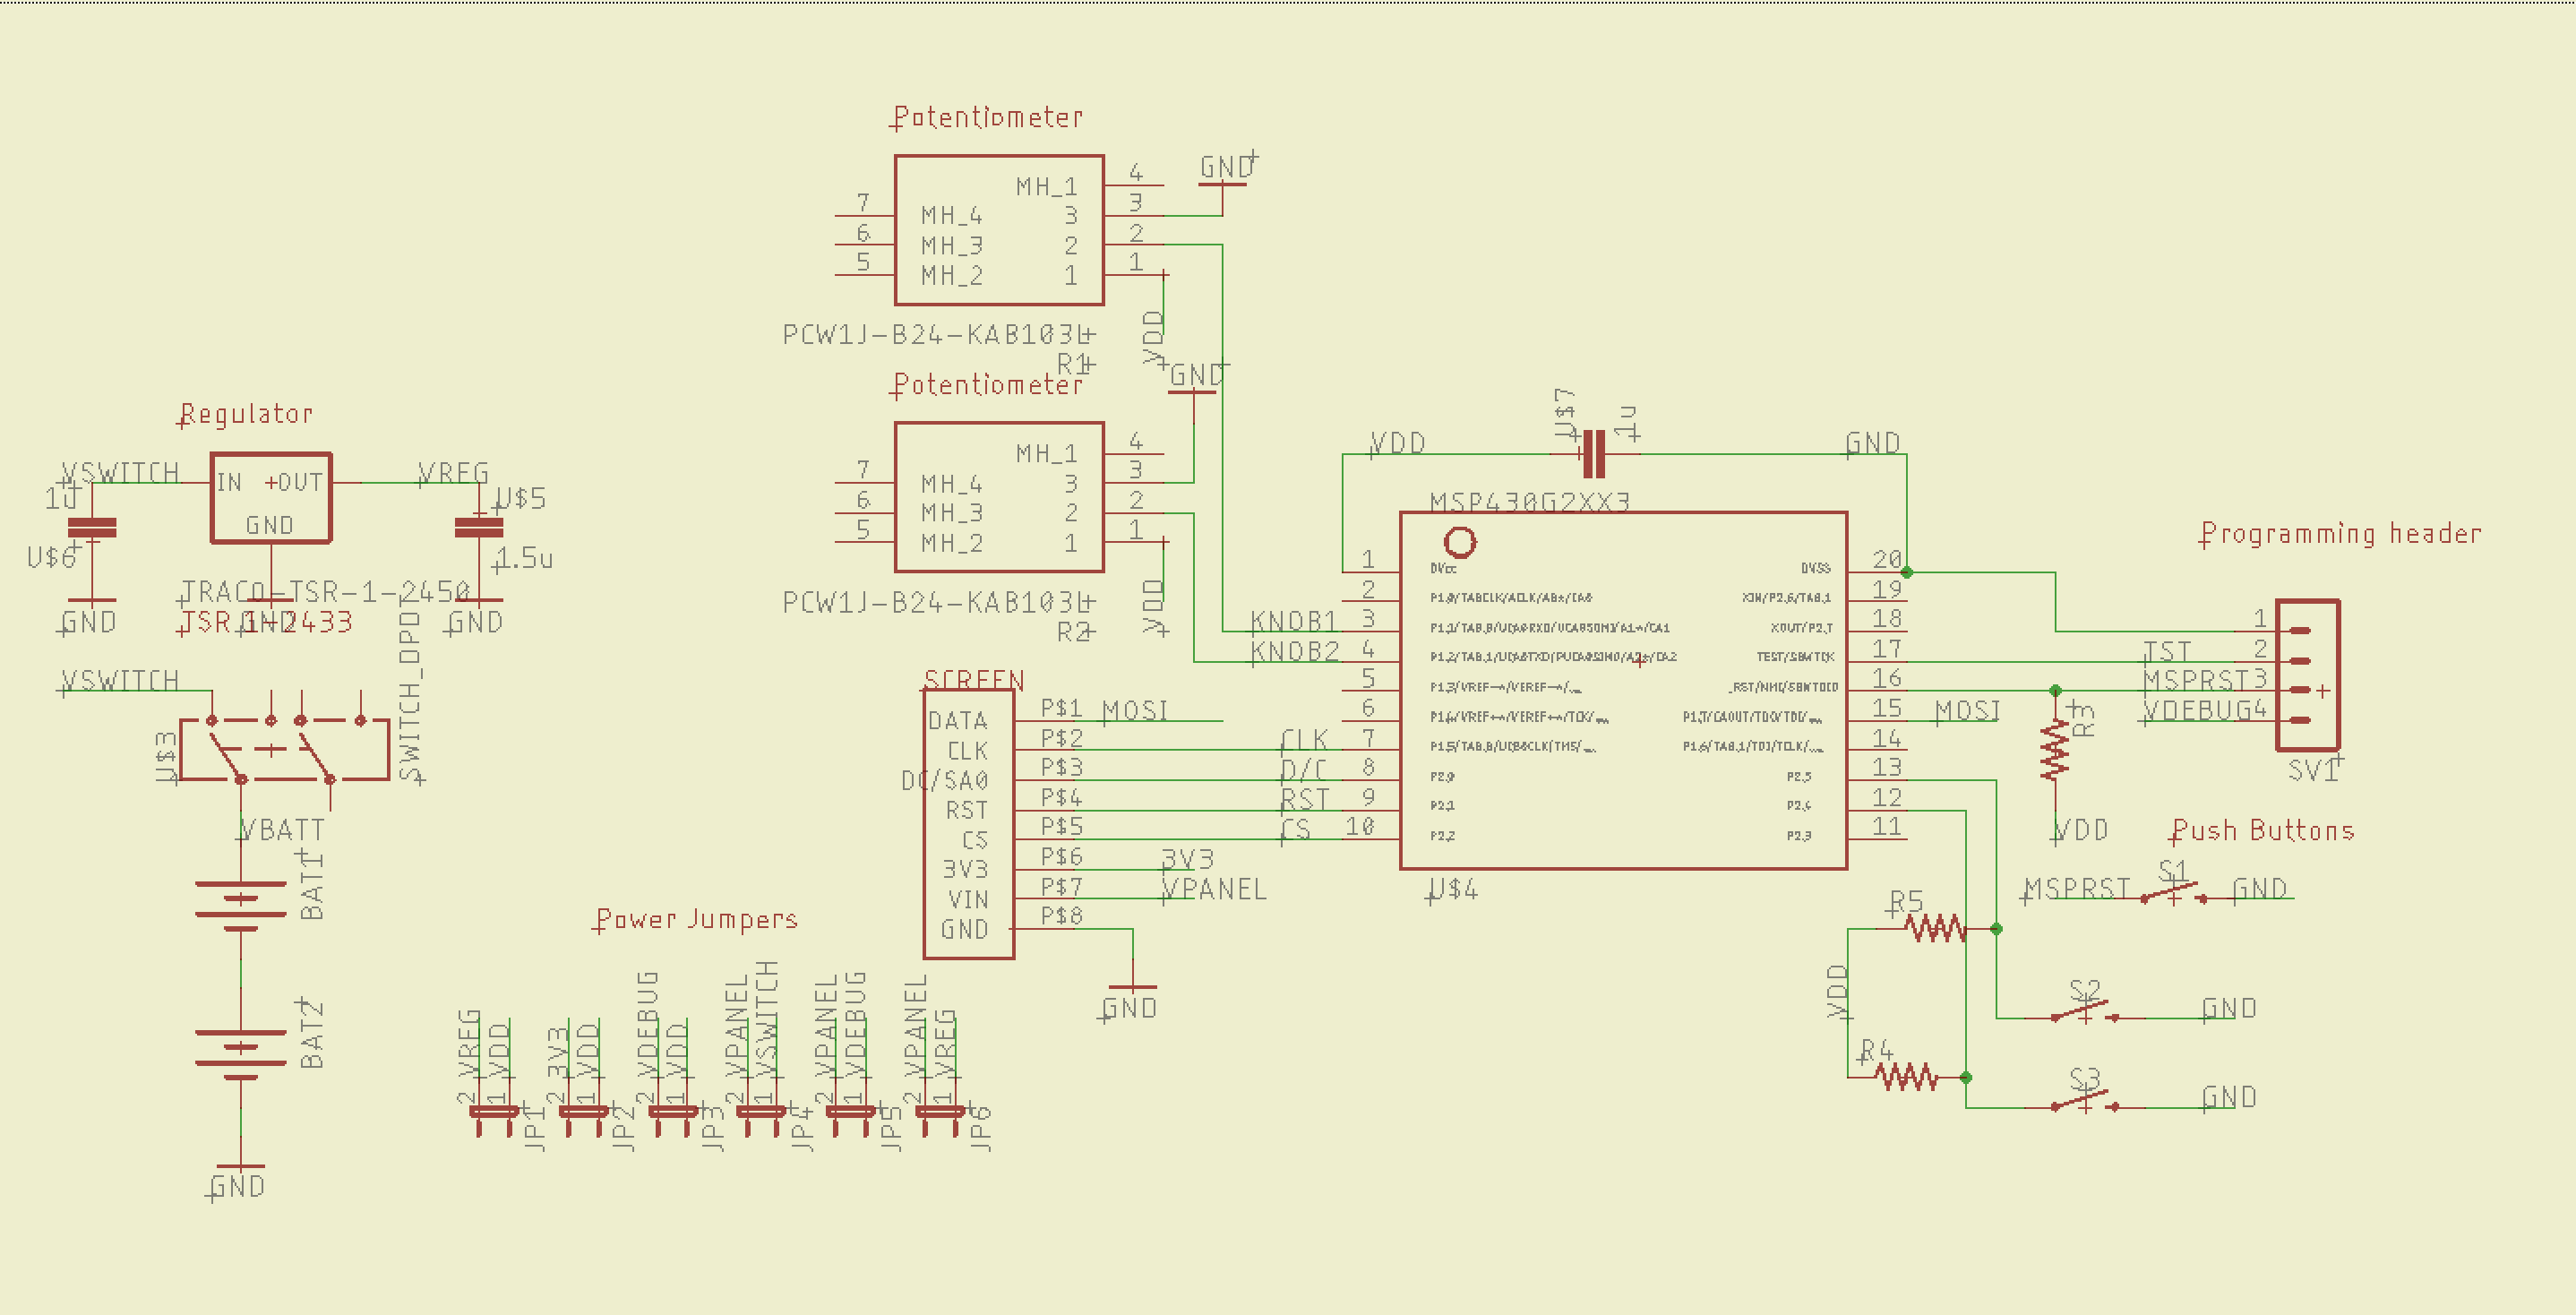
\includegraphics[height=0.6\textheight]{sch.png}
    \caption{Schematic.}
    \label{fig:PropProf}
\end{sidewaysfigure}

\begin{sidewaysfigure}[ht]
    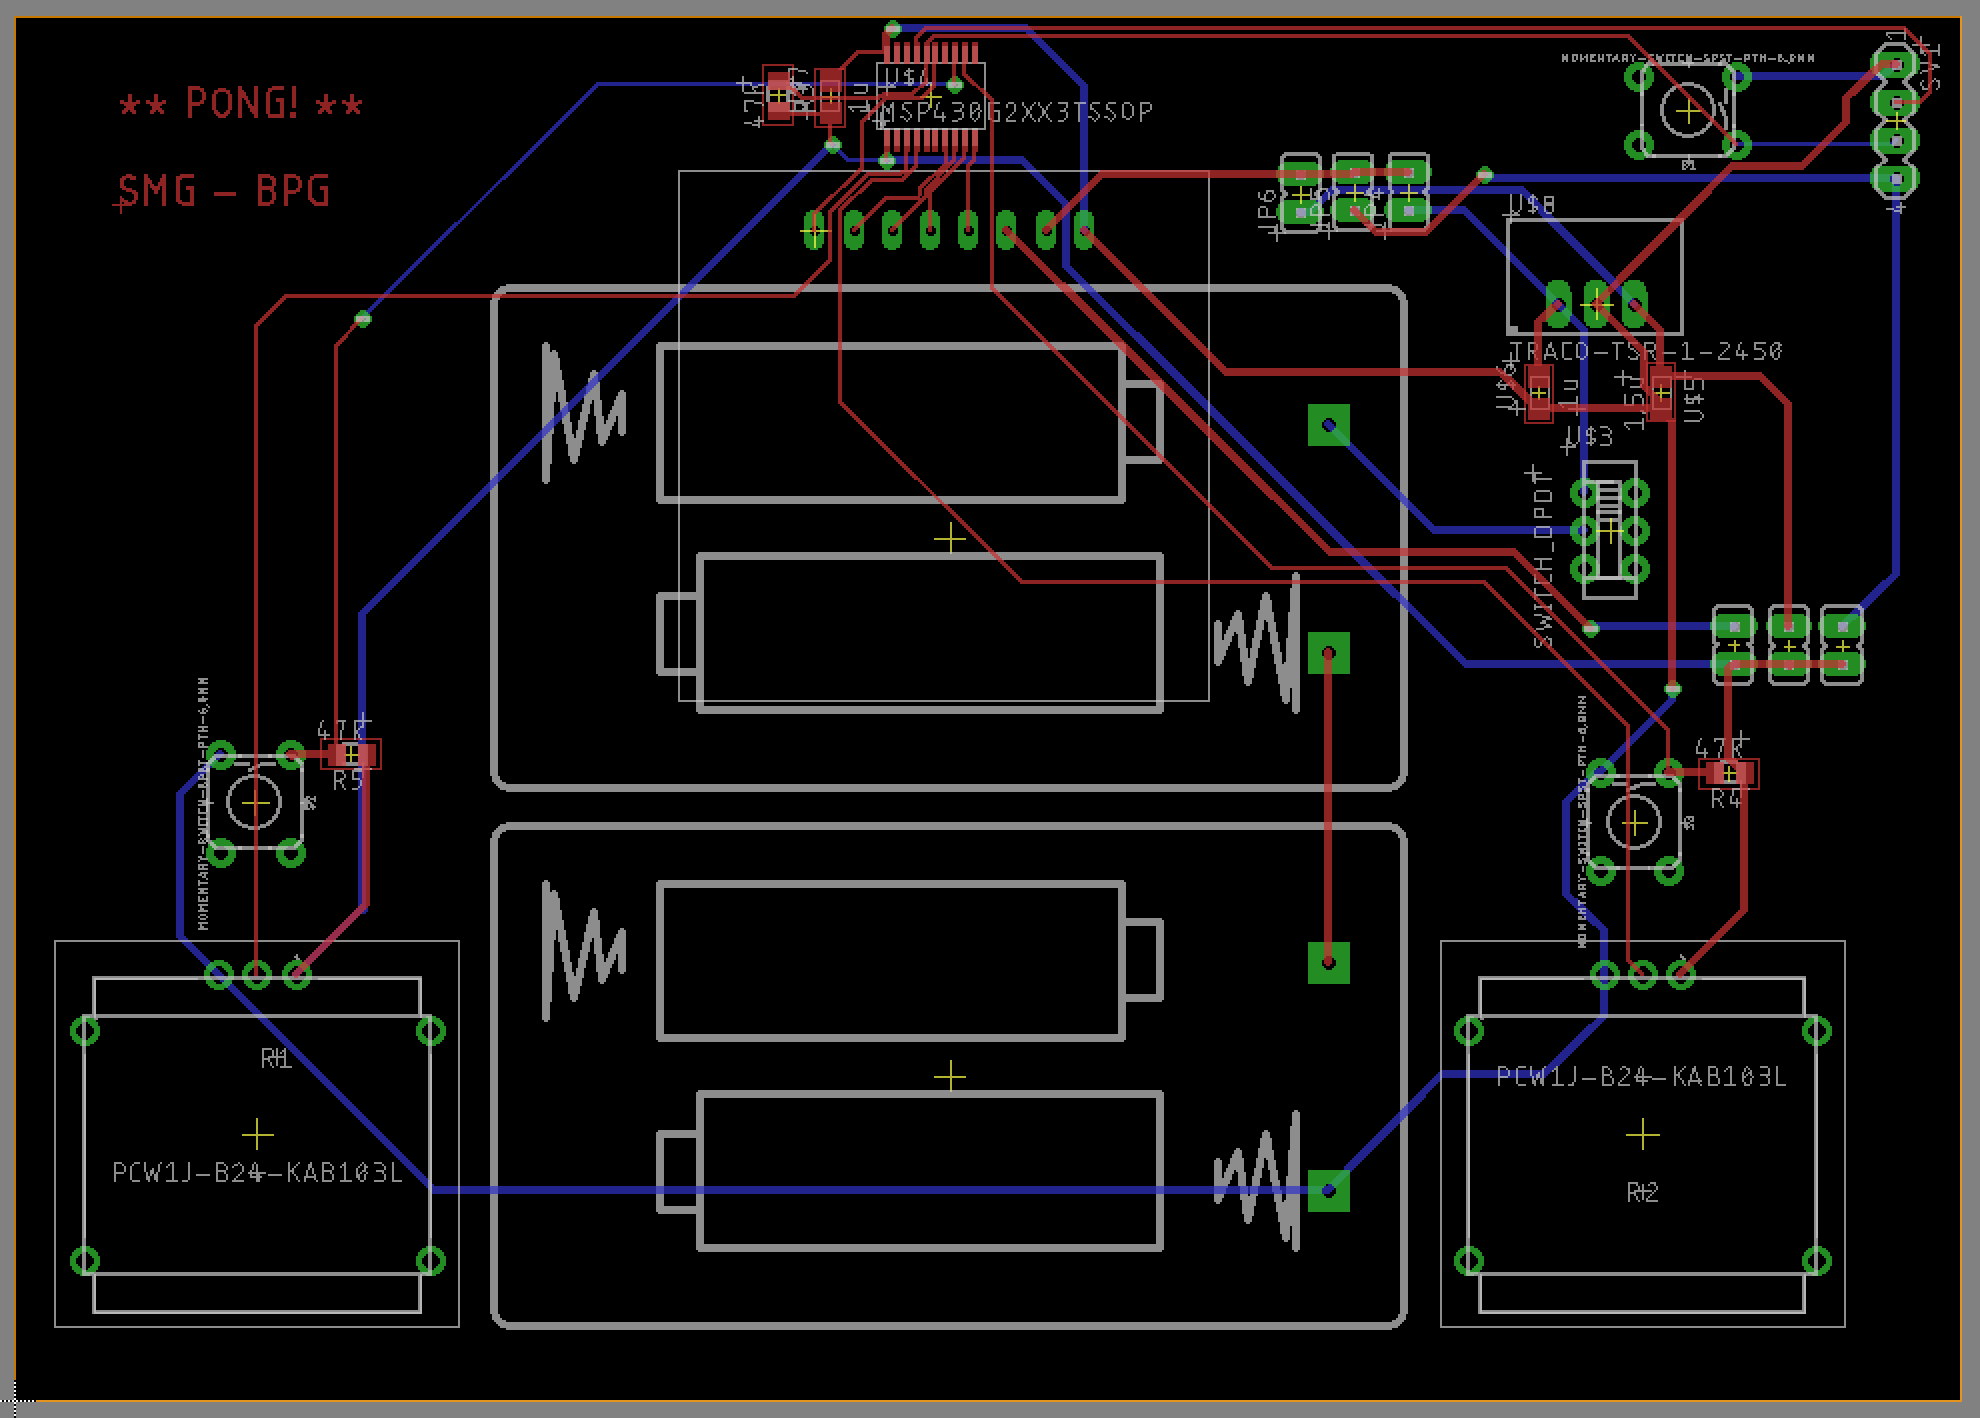
\includegraphics[height=0.8\textheight]{brd.png}
    \caption{Board layout.}
    \label{fig:PropProf}
\end{sidewaysfigure}

\end{document}
